\documentclass[12pt]{article}

\usepackage{amsmath}
\usepackage{amssymb}
\usepackage{physics}
\usepackage{enumitem}
\usepackage{geometry}
\geometry{margin=1in}
\usepackage{tikz}
\usetikzlibrary{angles,quotes,arrows.meta,calc,decorations.pathmorphing}

\begin{document}

\begin{center}
{\Large \textbf{FULL SYLLABUS TEST -- SET 1}}\\
\vspace{2mm}
(JEE Advanced Level -- Fully Audited Version)
\end{center}

\vspace{5mm}

\begin{enumerate}[leftmargin=0pt,itemindent=0pt]

%---------------- Q1 ----------------%

\item A smooth circular ring of radius $R$ lies in a vertical plane and rotates about its vertical diameter with constant angular speed $\omega$. A bead of mass $m$ carrying charge $q$ moves without friction on the ring. A uniform electric field $E$ acts vertically upward.

Let $\theta$ be measured from the lowest point. Assuming equilibrium occurs at non-zero $\theta$, the equilibrium condition obtained using effective potential in the rotating frame is:

\begin{enumerate}
\item[(A)] $m\omega^2R\sin\theta\cos\theta = mg\sin\theta - qE\cos\theta$
\item[(B)] $m\omega^2R\sin\theta = mg\cos\theta - qE\sin\theta$
\item[(C)] $m\omega^2R\sin\theta\cos\theta = mg\cos\theta + qE\sin\theta$
\item[(D)] $m\omega^2R\sin\theta = mg\sin\theta + qE\cos\theta$
\end{enumerate}

%---------------- Q2 ----------------%

\item A conducting rod of length $l$ and mass $m$ slides without friction on parallel rails inclined at angle $\theta$. The rails are connected by a resistor $R$. A uniform magnetic field $B$ acts vertically downward.

The terminal speed of the rod is:

\begin{center}
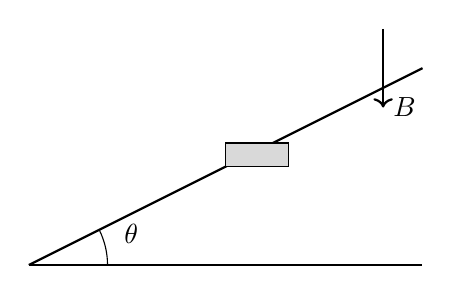
\begin{tikzpicture}[scale=1]
% Incline
\draw[thick] (0,0) -- (5,2.5);
\draw (0,0) -- (5,0);

% Angle marking
\draw (1,0) arc (0:26.5:1);
\node at (1.3,0.4) {$\theta$};

% Rod
\draw[fill=gray!30] (2.5,1.25) rectangle ++(0.8,0.3);

% Magnetic field downward
\draw[->,thick] (4.5,3) -- (4.5,2) node[right] {$B$};
\end{tikzpicture}
\end{center}

\begin{enumerate}
\item[(A)] $\dfrac{mg\sin\theta\,R}{B^2l^2}$
\item[(B)] $\dfrac{mgR}{B^2l^2}$
\item[(C)] $\dfrac{mg\sin\theta}{B^2l^2R}$
\item[(D)] $\dfrac{mgR\cos\theta}{B^2l^2}$
\end{enumerate}

%---------------- Q3 ----------------%

\item A solid sphere of radius $R$ rolls without slipping inside a smooth spherical bowl of radius $4R$.

For small oscillations about the lowest point, the angular frequency is:

\begin{enumerate}
\item[(A)] $\sqrt{\dfrac{5g}{14R}}$
\item[(B)] $\sqrt{\dfrac{7g}{10R}}$
\item[(C)] $\sqrt{\dfrac{10g}{7R}}$
\item[(D)] $\sqrt{\dfrac{14g}{5R}}$
\end{enumerate}

%---------------- Q4 ----------------%

\item A satellite moves in the central potential
\[
V(r) = -\frac{GMm}{r} + \frac{\alpha}{r^2}, \qquad \alpha \ll GMmR.
\]
If the circular orbit radius is $R$, the fractional change in angular frequency due to the perturbation term is:

\begin{enumerate}
\item[(A)] $\dfrac{\alpha}{GMmR}$
\item[(B)] $-\dfrac{\alpha}{GMmR}$
\item[(C)] $\dfrac{3\alpha}{2GMmR}$
\item[(D)] $-\dfrac{3\alpha}{2GMmR}$
\end{enumerate}

%---------------- Q5 ----------------%

\item A vertical column of ideal gas at uniform temperature $T$ is in a gravitational field $g$. The molar mass of the gas is $M$.

Find the ratio $\dfrac{P_{\text{bottom}}}{P_{\text{top}}}$ for a height difference $h$.

\begin{enumerate}
\item[(A)] $e^{\frac{Mg h}{RT}}$
\item[(B)] $e^{-\frac{Mg h}{RT}}$
\item[(C)] $1+\dfrac{Mg h}{RT}$
\item[(D)] $e^{\frac{RT}{Mg h}}$
\end{enumerate}

%---------------- Q6 ----------------%

\item A uniform rod of length $L$ and mass $m$ is pivoted at one end. A charge $+q$ is fixed at its free end. A point charge $+Q$ is fixed horizontally at a distance $L$ from the pivot.

For small oscillations in a vertical plane, the angular frequency is:

\begin{center}
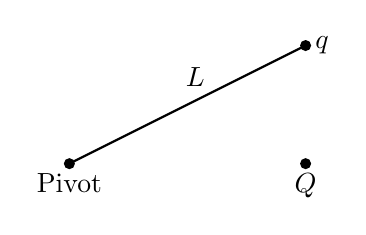
\begin{tikzpicture}[scale=1]
% Pivot
\fill (0,0) circle (2pt);
\node[below] at (0,0) {Pivot};

% Rod
\draw[thick] (0,0) -- (3,1.5);

% Charge at end
\fill (3,1.5) circle (2pt);
\node[right] at (3,1.5) {$q$};

% External charge
\fill (3,0) circle (2pt);
\node[below] at (3,0) {$Q$};

% Length label
\node at (1.6,1.1) {$L$};
\end{tikzpicture}
\end{center}

\begin{enumerate}
\item[(A)] $\sqrt{\dfrac{3g}{2L}+\dfrac{kqQ}{mL^3}}$
\item[(B)] $\sqrt{\dfrac{3g}{2L}-\dfrac{kqQ}{mL^3}}$
\item[(C)] $\sqrt{\dfrac{g}{L}+\dfrac{kqQ}{mL^3}}$
\item[(D)] $\sqrt{\dfrac{3g}{L}+\dfrac{kqQ}{2mL^3}}$
\end{enumerate}

%---------------- Q7 ----------------%

\item In Young’s double slit experiment, slit separation is $d$, screen distance is $D$, and wavelength is $\lambda$. A thin plate of refractive index $\mu$ and thickness $t$ is introduced in front of one slit.

The shift of the central maximum on the screen is: 

\begin{center}
\begin{tikzpicture}[scale=1]
% Slits
\draw[thick] (0,1) -- (0,0.7);
\draw[thick] (0,-0.7) -- (0,-1);

% Thin plate on upper slit
\draw[fill=gray!30] (0.1,0.7) rectangle (0.4,1);

% Screen
\draw[thick] (6,2) -- (6,-2);
\node[right] at (6,0) {Screen};

% Rays
\draw (0,0.85) -- (6,0.5);
\draw (0,-0.85) -- (6,-0.5);

\node at (0.3,1.3) {Plate};
\end{tikzpicture}
\end{center}


\begin{enumerate}
\item[(A)] $\dfrac{D(\mu-1)t}{d}$
\item[(B)] $\dfrac{Dt}{d}$
\item[(C)] $\dfrac{D\lambda(\mu-1)}{d}$
\item[(D)] $\dfrac{t(\mu-1)}{\lambda}$
\end{enumerate}

%---------------- Q8 ----------------%

\item A charged particle of mass $m$ and charge $q$ enters a region where a magnetic field $B$ is into the page and an electric field $E$ is horizontal. The initial velocity is horizontal and perpendicular to $B$.

If $E = 2vB$, the radius of trajectory is:

\begin{center}
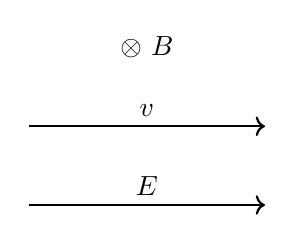
\begin{tikzpicture}[scale=1]
% Velocity
\draw[->,thick] (0,0) -- (3,0);
\node[above] at (1.5,0) {$v$};

% Electric field
\draw[->,thick] (0,-1) -- (3,-1);
\node[above] at (1.5,-1) {$E$};

% Magnetic field into page
\node at (1.5,1) {$\otimes\ B$};
\end{tikzpicture}
\end{center}

\begin{enumerate}
\item[(A)] $\dfrac{m}{qB}$
\item[(B)] $\dfrac{mv}{qB}$
\item[(C)] $\dfrac{m}{2qB}$
\item[(D)] Straight line
\end{enumerate}

%---------------- Q9 ----------------%

\item A piston of area $A$ contains ideal gas at equilibrium pressure $P$ and length $L$. A spring of constant $k$ is attached to the piston. The mass of the piston is $M$.

For small adiabatic oscillations (ratio of specific heats $\gamma$), the angular frequency is:

\begin{center}
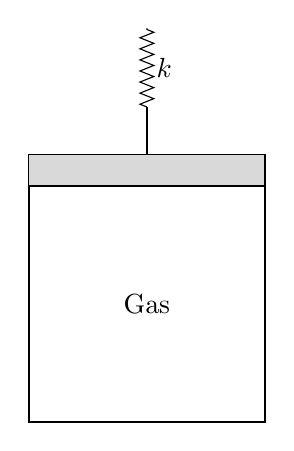
\begin{tikzpicture}[scale=1]
% Container
\draw[thick] (0,0) rectangle (3,3);

% Gas label
\node at (1.5,1.5) {Gas};

% Piston
\draw[fill=gray!30] (0,3) rectangle (3,3.4);

% Spring
\draw[thick] (1.5,3.4) -- (1.5,4);
\draw[decorate,decoration={zigzag,segment length=4pt}] (1.5,4) -- (1.5,5);
\node[right] at (1.5,4.5) {$k$};
\end{tikzpicture}
\end{center}

\begin{enumerate}
\item[(A)] $\sqrt{\dfrac{k+\gamma PA/L}{M}}$
\item[(B)] $\sqrt{\dfrac{k+PA/L}{M}}$
\item[(C)] $\sqrt{\dfrac{\gamma PA}{M}}$
\item[(D)] $\sqrt{\dfrac{k}{M}}$
\end{enumerate}

%---------------- Q10 ----------------%

\item A block of mass $m$ carrying charge $q$ slides down a rough incline of angle $\theta$. A magnetic field $B$ is perpendicular to the plane. Coefficient of friction is $\mu$. If its velocity is $v$, the acceleration down the plane is:

\begin{center}
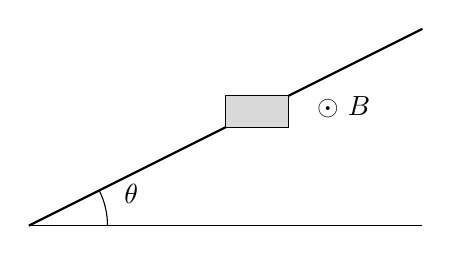
\begin{tikzpicture}[scale=1]
% Incline
\draw[thick] (0,0) -- (5,2.5);
\draw (0,0) -- (5,0);

% Angle
\draw (1,0) arc (0:26.5:1);
\node at (1.3,0.4) {$\theta$};

% Block
\draw[fill=gray!30] (2.5,1.25) rectangle ++(0.8,0.4);

% Magnetic field out of plane
\node at (4,1.5) {$\odot\ B$};
\end{tikzpicture}
\end{center}

\begin{enumerate}
\item[(A)] $g\sin\theta$
\item[(B)] $g\sin\theta-\mu g\cos\theta$
\item[(C)] $g\sin\theta-\mu\left(g\cos\theta+\dfrac{qvB}{m}\right)$
\item[(D)] $g\sin\theta+\dfrac{qvB}{m}$
\end{enumerate}

%---------------- Q11 ----------------%

\item A hydrogen atom is placed in a uniform magnetic field $B$. Consider the normal Zeeman effect for a transition with $\Delta m_l = 1$.

The energy splitting is:

\begin{enumerate}
\item[(A)] $\mu_B B$
\item[(B)] $2\mu_B B$
\item[(C)] $\dfrac{\mu_B B}{2}$
\item[(D)] $\dfrac{eB}{m_e}$
\end{enumerate}

%---------------- Q12 ----------------%

\item In a series RLC circuit with ideal $L$ and $C$, the resonance angular frequency is:

\begin{enumerate}
\item[(A)] $\dfrac{1}{\sqrt{LC}}$
\item[(B)] $\sqrt{\dfrac{L}{C}}$
\item[(C)] $\dfrac{R}{L}$
\item[(D)] $\sqrt{\dfrac{R^2}{LC}}$
\end{enumerate}

%---------------- Q13 ----------------%

\item A satellite is in a circular orbit of radius $r$ around Earth. It is given a small tangential impulse so that it just escapes the gravitational field.

The escape speed from that orbit is:

\begin{enumerate}
\item[(A)] $\sqrt{\dfrac{2GM}{r}}$
\item[(B)] $\sqrt{\dfrac{GM}{r}}$
\item[(C)] $\sqrt{\dfrac{GM}{2r}}$
\item[(D)] $\dfrac{1}{2}\sqrt{\dfrac{2GM}{r}}$
\end{enumerate}

%---------------- Q14 ----------------%

\item Two capacitors $C$ and $2C$ are connected in series with a battery $V$. A dielectric of constant $K$ is inserted fully in capacitor $C$.

The ratio of new to initial energy $\dfrac{U'}{U}$ is:

\begin{enumerate}
\item[(A)] $\dfrac{2K}{K+2}$
\item[(B)] $\dfrac{K+2}{2K}$
\item[(C)] $\dfrac{K}{K+2}$
\item[(D)] $\dfrac{2}{K+2}$
\end{enumerate}

%---------------- Q15 ----------------%

\item A bead of mass $m$ moves on a vertical circular track of radius $R$. It is projected from the bottom with speed $u$.

The normal reaction at the highest point is:

\begin{center}
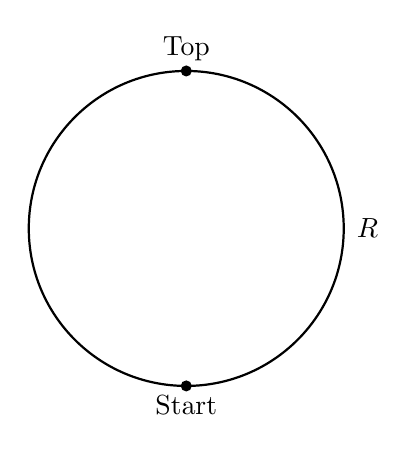
\begin{tikzpicture}[scale=1]
% Circle
\draw[thick] (0,0) circle (2);

% Bottom and top
\fill (0,-2) circle (2pt);
\fill (0,2) circle (2pt);

\node[below] at (0,-2) {Start};
\node[above] at (0,2) {Top};

\node at (2.3,0) {$R$};
\end{tikzpicture}
\end{center}
\begin{enumerate}
\item[(A)] $\dfrac{mu^2}{R}-5mg$
\item[(B)] $\dfrac{mu^2}{R}-mg$
\item[(C)] $\dfrac{mu^2}{R}-3mg$
\item[(D)] $\dfrac{mu^2}{R}+mg$
\end{enumerate}

\end{enumerate}

\end{document}